% !TEX root = main.tex

%%%%%%%%%%%%%%%%%%%%%%%%%%%%%%%%%%%%%%%%%%%%%%%%%%%%%%%%%%%%%%%%%%%%%%%%%%%%%%%%%%%%%%%%%%%%%%%%
\section{宿題}
%%%%%%%%%%%%%%%%%%%%%%%%%%%%%%%%%%%%%%%%%%%%%%%%%%%%%%%%%%%%%%%%%%%%%%%%%%%%%%%%%%%%%%%%%%%%%%%%

\begin{enumerate}
    \item サイリスタ(SCR)の動作原理を調べよ.
    \begin{description}
        \item[] サイリスタは,ゲート(G)からカソード(K)にゲート電流を流すことにより,
        アノード(A)とカソード(K)間を導通させることができる3端子の整流素子である.
        図4(a)はサイリスタの簡単な構造図で,P型,N型,P型,N型の順に半導体
        を接合した4層構造で,途中のP型半導体にゲート端子を取り付けた構造になっている.
        また,サイリスタは,図4(b)のように,PNPトランジスタとNPNトランジスタ
        とを組み合わせた複合回路としてみることができる.
        \begin{figure}[H]
            \begin{center}
                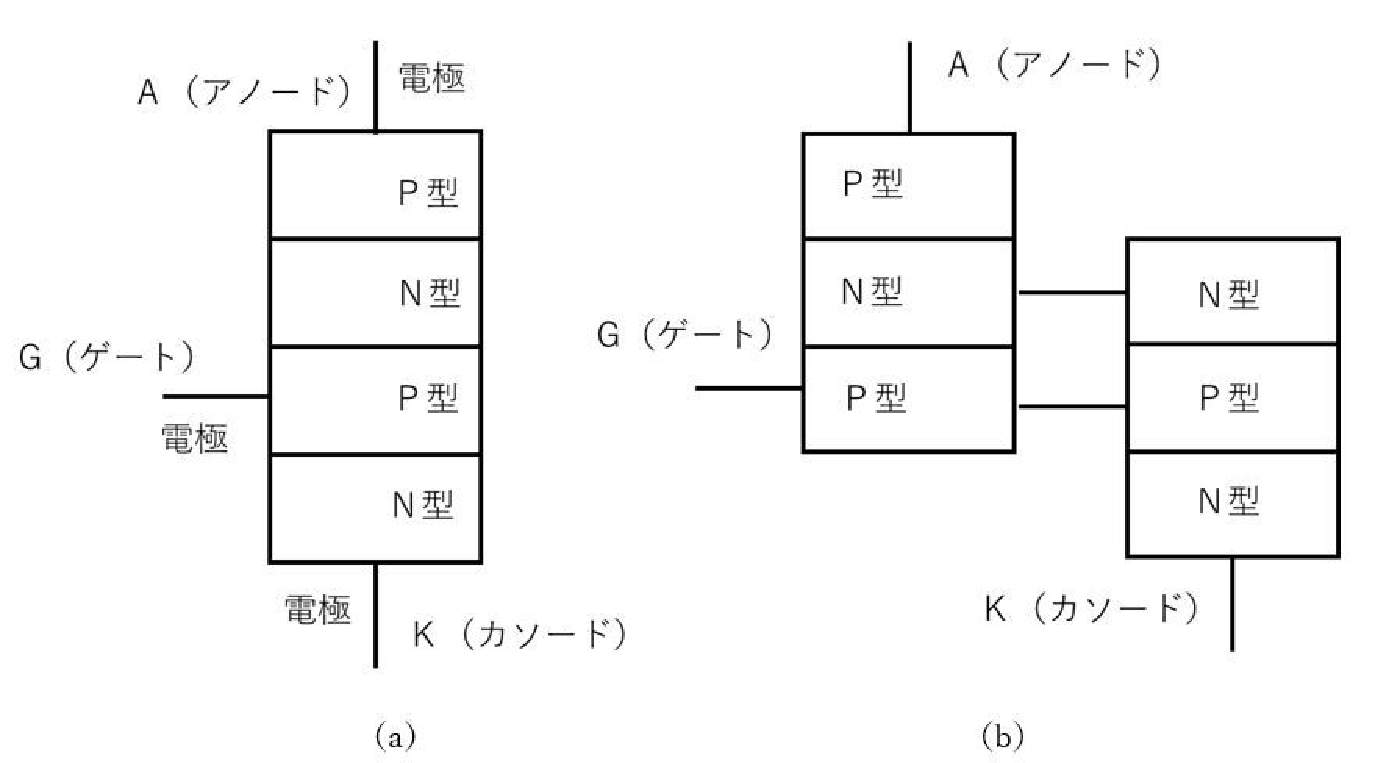
\includegraphics[scale=0.5]{figure4.pdf}
                \caption{サイリスタの構造イメージ}
            \end{center}
        \end{figure}

        ゲート(G)に電流が流れない場合($I_G=0$)には,$Tr2$はOFF状態になっていて
        Tr2のコレクタには電流($I_{C2}$)は流れない.そのため,$Tr1$のベース
        ($I_{B1}$)にも電流は流れず,$Tr1$もOFFの状態になっている.
        この状態ではアノード(A)に電圧が加わってもサイリスタの電流は流れない.
        \begin{figure}[H]
            \begin{center}
                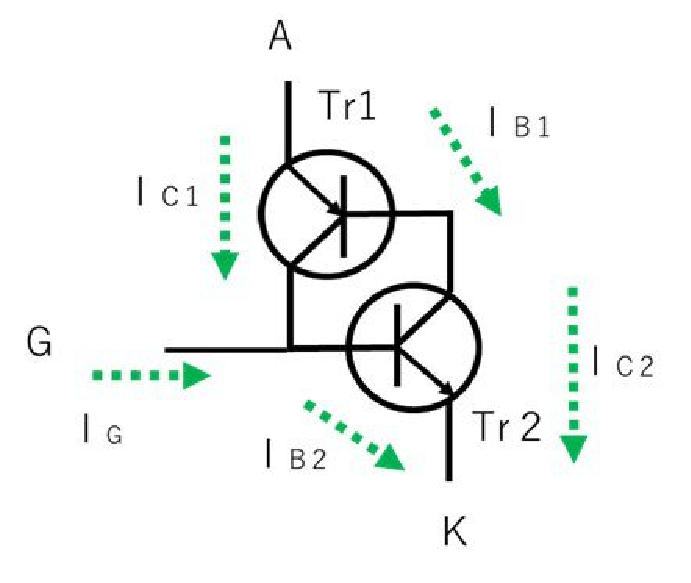
\includegraphics[scale=0.5]{figure5.pdf}
                \caption{サイリスタの基本動作}
            \end{center}
        \end{figure}

        \newpage

        ゲート(G)すなわち$Tr2$のベースに電流($I_G$)が流れた場合,$Tr2$は
        ON状態になる.これにより$Tr2$のコレクタを通して$Tr1$のベース電流
        ($I_{B1}$)が流れる.$Tr1$にベース電流が流れるので,$Tr1$はON状態になる.
        そして,$Tr1$のコレクタを通して$Tr2$のベースに電流($I_{B2}$)が流れる.
        
        $Tr1$から$Tr2$のベースに電流が流れるので,ゲートの電流が無くなっても
        サイリスタのアノード(A)側からカソード(K)側には電流が流れ続ける.
        これを「自己保持状態」という.

        また,導通状態を停止させるには,アノード(A)とカソード(K)間の電流を
        一定値以下に下げることが必要である.
        \begin{figure}[H]
            \begin{center}
                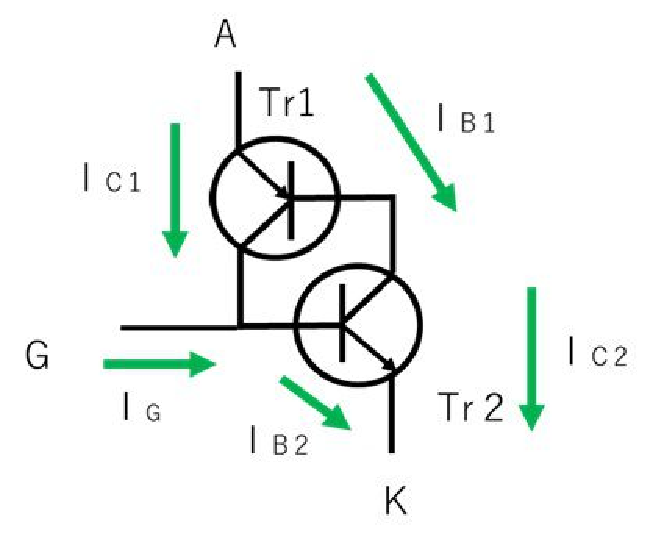
\includegraphics[scale=0.5]{figure6.pdf}
                \caption{自己保持状態}
            \end{center}
        \end{figure}

    \end{description}
\end{enumerate}